\section{Umsetzung des Equilibrium-Propagation in Simulink}
\label{app:Umsetzung des Equilibrium-Propagation in Simulink}

In Abbildung \ref{fig:EqProp Discrete Simulink} ist ein diskreter Ansatz in Simulink für \ac{ep} zu sehen, der sich durch den "`Memory"'-Block (dargestellt durch den rotierenden Pfeil) auszeichnet. Da dieser Block den jeweils letzten Eingabewert speichert und diese Funktion nicht auf analoge Rechner übertragbar ist, kann dieser Ansatz praktisch nicht umgesetzt werden.

\begin{figure}[h]
  \label{fig:EqProp Discrete Simulink}
  \caption{Umsetzung eines diskreten Ansatzes zur Lösung des \ac{ep} in Simulink}
  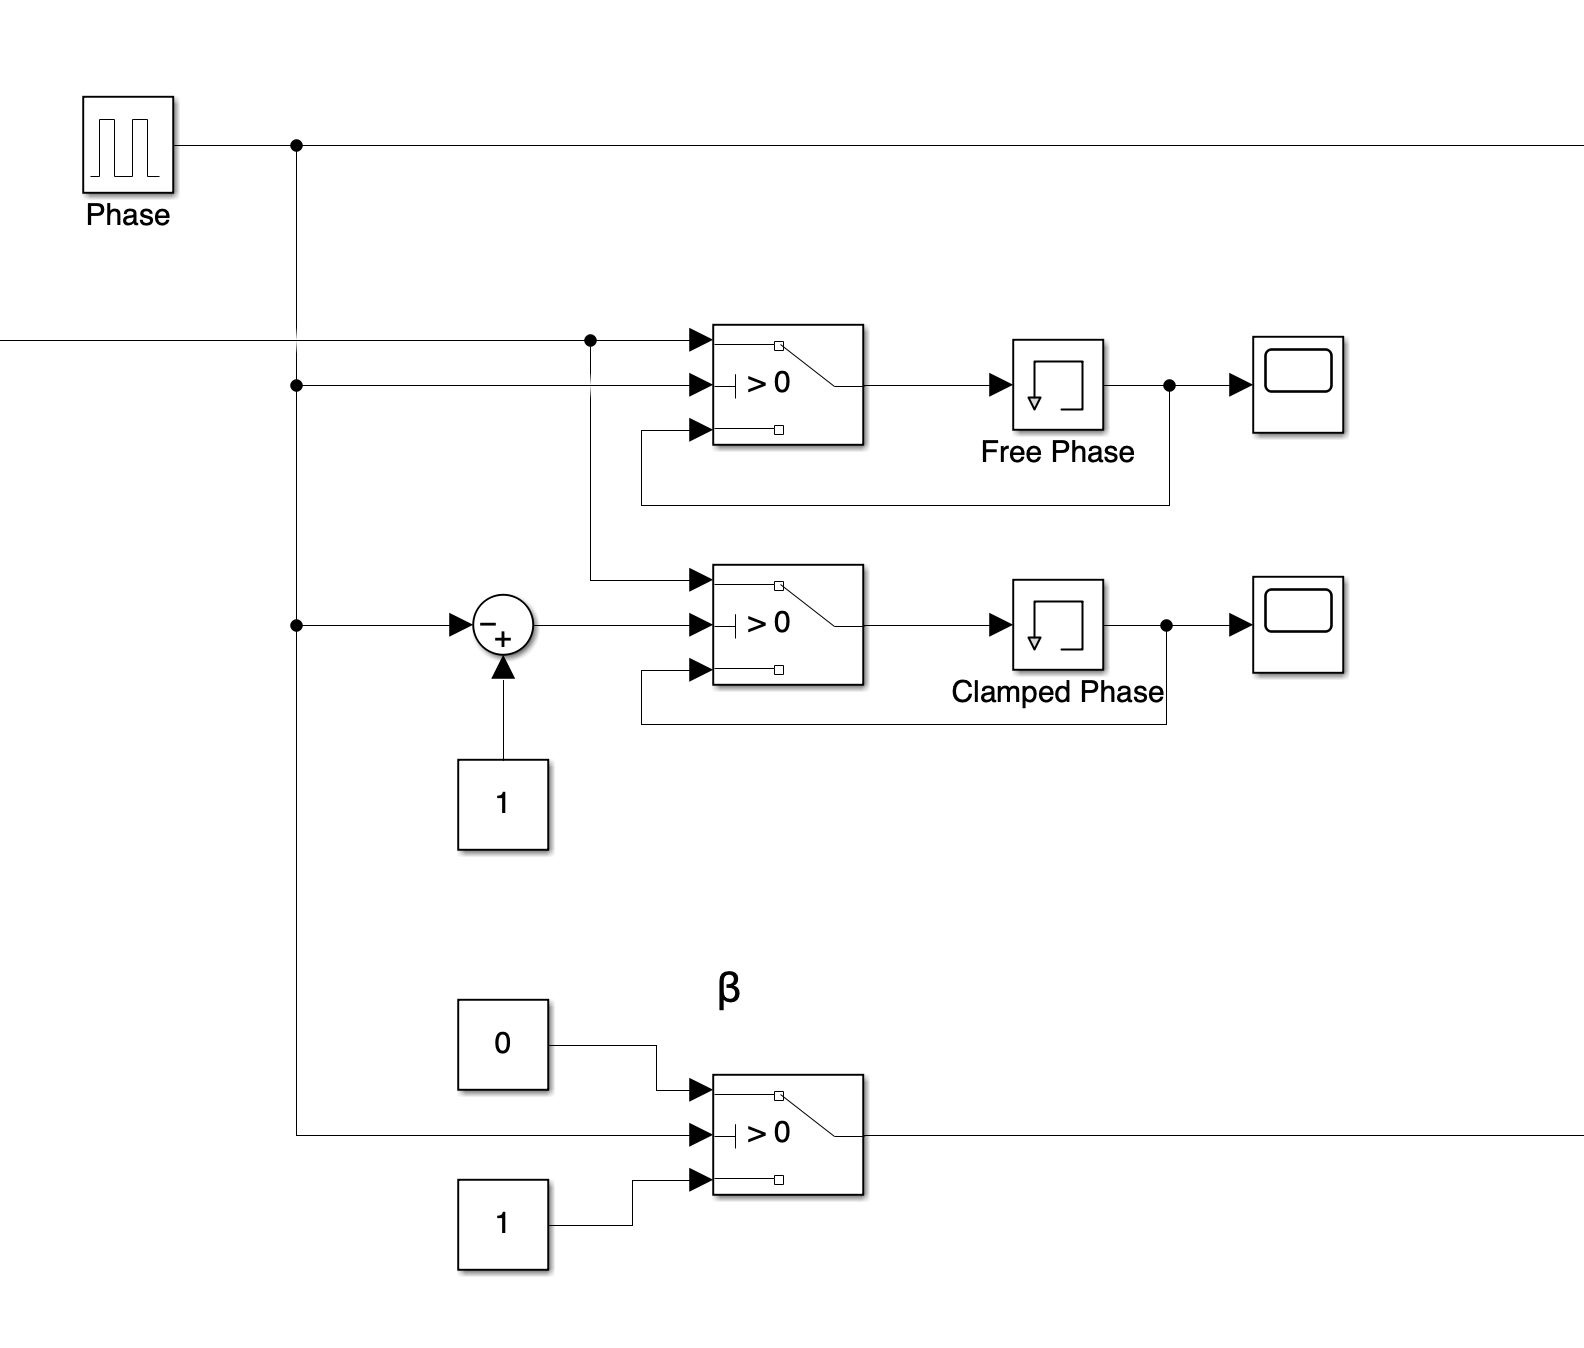
\includegraphics[width=\textwidth]{abbildungen/ep_discrete_simulink.png}
  \\
  Quelle: Eigene Darstellung
\end{figure}

Das \ac{c-ep} wurde in Simulink für ein \ac{hnn} mit drei Neuronen und damit drei Gewichten modelliert und ist in Abbildung \ref{fig:C-EP Simulink} dargestellt.

\begin{figure}[h]
  \label{fig:C-EP Simulink}
  \caption{Umsetzung einer Annäherung an \ac{c-ep} in Simulink}
  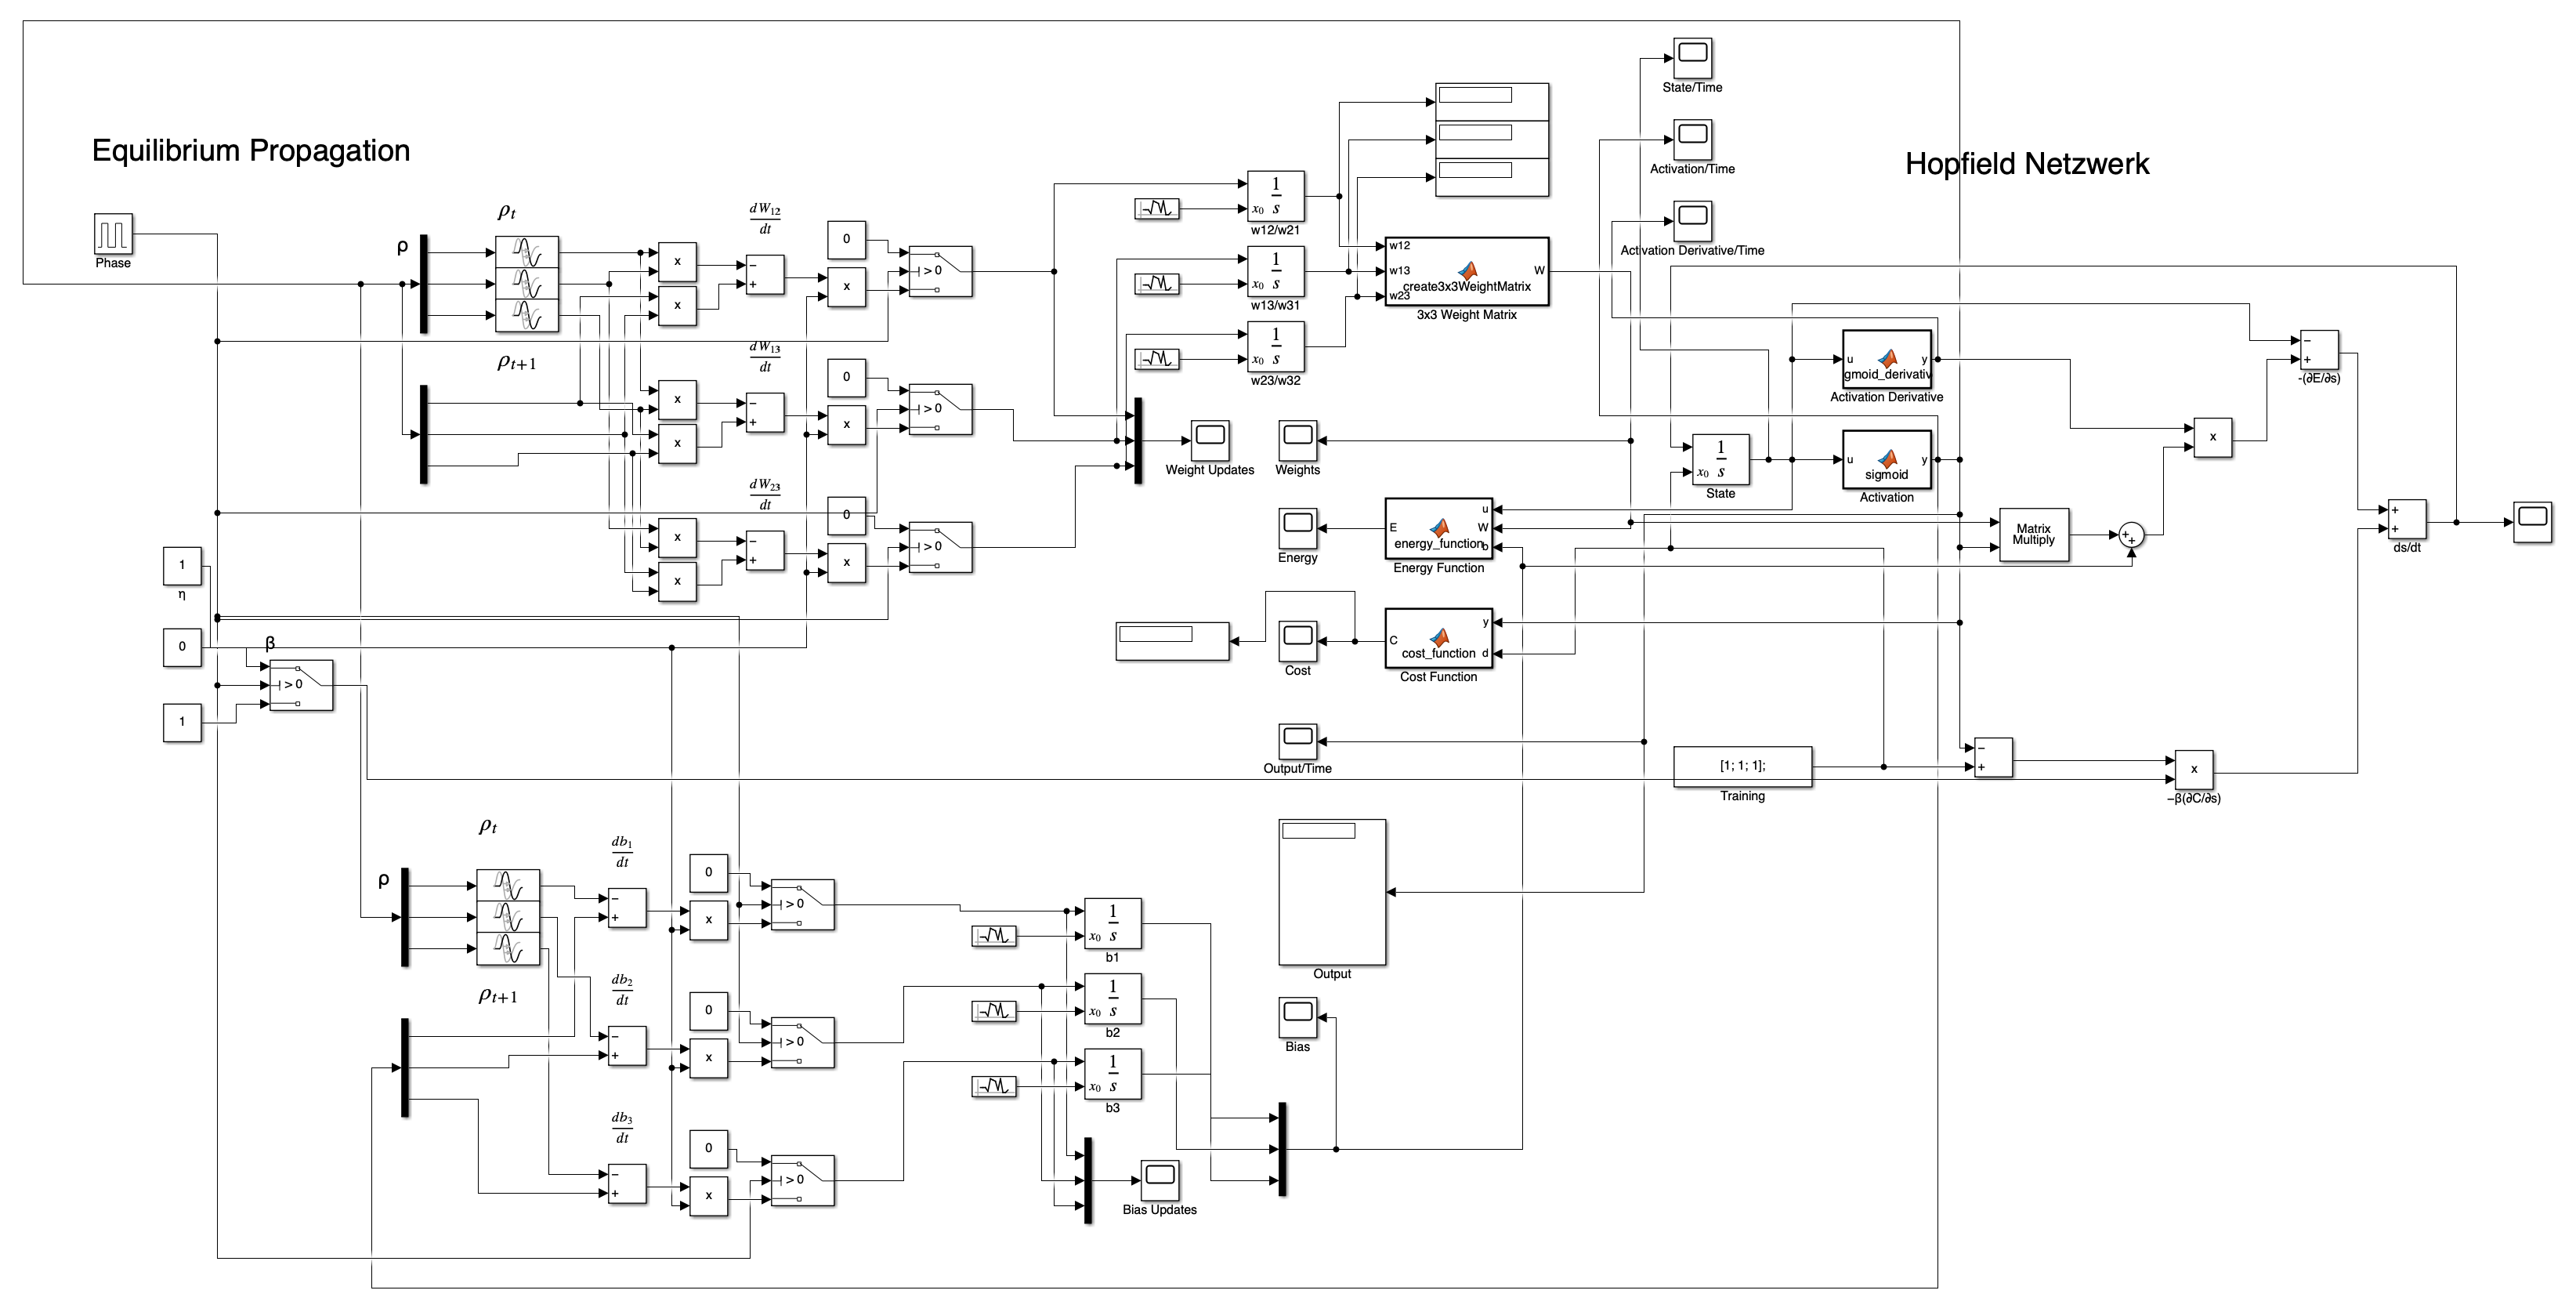
\includegraphics[width=\textwidth]{abbildungen/c-ep_simulink.png}
  \\
  Quelle: Eigene Darstellung
\end{figure}

Um den Zeitaufwand durch die Konstruktion eines größeren Modells des \ac{c-ep} für größere Netzwerke zu sparen, wurde die Simulation mit sechs Neuronen aus \ref{chap:Validierung des Algorithmus durch Testläufe} mithilfe des in Abbildung \ref{fig:C-EP Sim Simulink} durchgeführt. Dieses Modell nutzt Matlab Funktionsblöcke, um Eingabewerte in Form von Vektoren bzw. Matrizen beliebiger Größe verarbeiten zu können.

\begin{figure}[h]
  \label{fig:C-EP Sim Simulink}
  \caption{Größere Simulationen des \ac{c-ep} können mithilfe der Matlab-Funktionsblöcke in Simulink durchgeführt werden, um Aufwand beim Modellieren zu sparen.}
  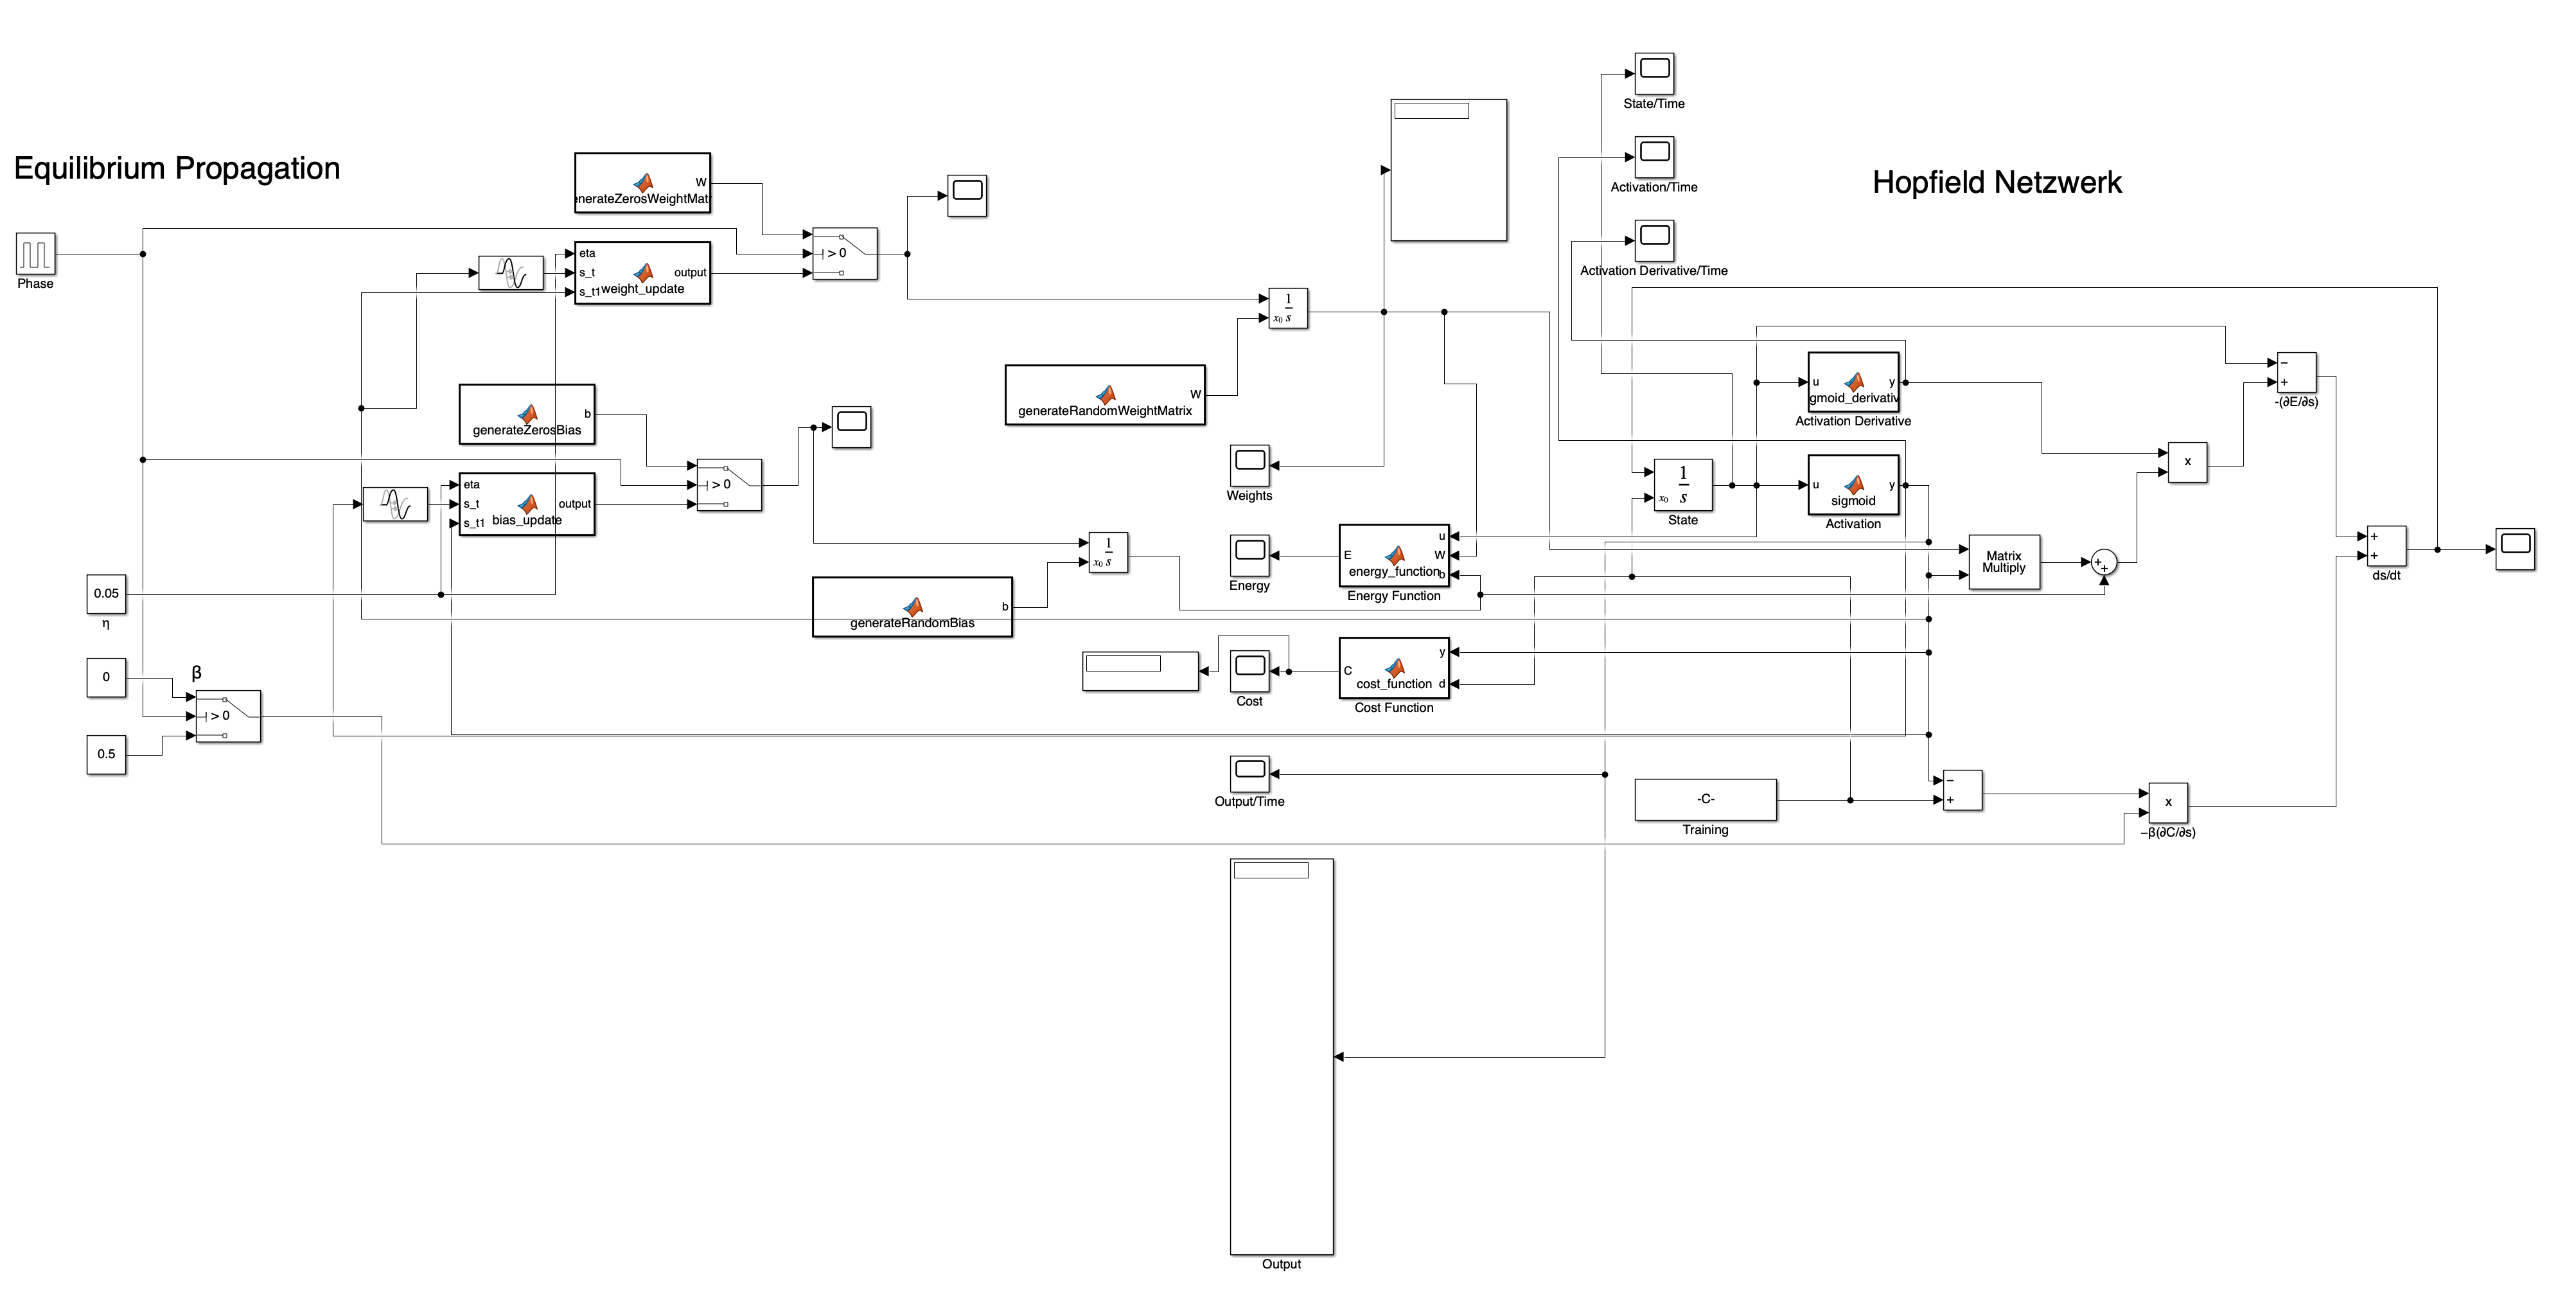
\includegraphics[width=\textwidth]{abbildungen/c-ep_sim_simulink.png}
  \\
  Quelle: Eigene Darstellung
\end{figure}
